\documentclass[]{article}
\usepackage{graphicx}
\usepackage{float}
\usepackage{tikz}
\usepackage{amsmath}
\usepackage{multirow}
\usepackage{subcaption}
\usetikzlibrary{arrows}

%opening
\begin{document}
	\section{Donald Knuth's Mastermind}
		Donald Knuth's algorithm for solving the classic (6,4) Mastermind, published in 1977, showed that the codemaker can always win in five moves or fewer. The algorithm works on a mini-max approach.
		
		The "best" initial guess has been shown to be (1, 1, 2, 2), and it was shown that other initial guesses might not provide the guarantee of 5 or fewer guesses for finishing the game. Each step in the algorithm involves eliminating the codes that are not consistent with the ones that have been guessed, from the set of possible 1296 codes (say $S$), thereby reducing the search space.
		The next step involves providing a "score" to \textit{all of the possible codes}. The score given to a code the minimum number of possibilities it might eliminate from $S$. This subroutine requires $1296 \times |S_t|$ number of iterations, where $t$ is the current number of guesses, and $|S_t|$ denotes the reduced set after $t$ guesses. The mini-max approach comes into play when the code with the maximum score is used as our next guess.	
		
		An interesting aspect of Knuth's algorithm is that it does not require the guesses to be consistent with the previous guesses. The algorithm works on the basis of maximizing reduction in the set size, and can guess inconsistent codes to cut down on the search space. However, due to the large number of possible codes and the notion of multiple passes through the set, Knuth's algorithm performs well in theory to minimize number of guesses, but does not perform well in terms of time. Hence, we look for a better approach that can balance optimality of guesses along with time.

\begin{figure}[H]
		\centering
		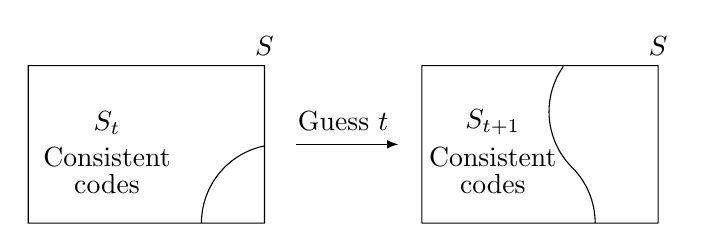
\begin{tikzpicture}
			\draw (1.2,0) arc[start angle=180, end angle=101, radius=1] (-0, 1) node [text=black,above] {$S_t$}
			(-0, 0.6) node [text=black,above] {Consistent}
			(-0, 0.25) node [text=black,above] {codes}
			(-1,0) rectangle (2,2) node [text=black,above] {$S$};
			
			\draw [-latex] (2.4,1) -- (3.7,1);
			\draw (3, 1.05) node [text=black,above] {Guess $t$};
			    
			\draw (6.2,0) arc[start angle=0, end angle=45, radius=1] 
			(4.9, 1) node [text=black,above] {$S_{t+1}$}
			(4.9, 0.6) node [text=black,above] {Consistent}
			(4.9, 0.25) node [text=black,above] {codes}
			(5.907, 0.707) arc[start angle=225, end angle=145, radius=1]
			(4,0) rectangle (7,2) node [text=black,above] {$S$};
		\end{tikzpicture}
		\caption{Reducing consistent combination search space}
\end{figure}
\end{document}